
\chapter{Introduction to the Standard Model}
\label{Chapter 1} 
\captionsetup{justification=justified,singlelinecheck=false}

\lhead{Chapter 1. \emph{The Standard Model}} 



When great minds of science such as Galileo, Newton and Kepler turned their attention to understanding the world and the operations of nature, a whole new beauty unfolded -- a beauty of mathematical precision and simplicity. In a single concise statement Kepler accurately described not just the motion of a single planet but that of all planets. Newton with his Second Law now more tersely written as ${\bf{F}}=m{\bf{a}}$, captured the essential motion of all macroscopic bodies. Mankind is naturally attracted to simplicity, and concise statements explaining a large body of seemingly diverse phenomena are considered beautiful. Perhaps the more concise or fundamental a given statement is and the more diverse the phenomena that are encapsulated in that statement, the more beauty it holds and value it is given in the scientific community. 

A whole branch of physics developed in the 20th century called particle physics focused on understanding the fundamental particles which constitute the universe. Progress in this field advanced along with new particle discoveries, some predicted and some a surprise. After Planck had beautifully ``fixed'' the ultraviolet divergences of statistical mechanics analysis of blackbody radiation, Einstein took the concept a step further and proposed a fully quantized electromagnetic field, explaining the observed photo-electric in terms of a quantum particle called the ``photon''. Rutherford's work with alpha rays had proven that all elemental nuclei contained the hydrogen nucleus and by 1920 this particle was being termed the ``proton''. A decade later under the direction of Rutherford, James Chadwick discovered evidence of a second nucleon which had almost the same mass as the proton but which was electrically neutral. Around the same time, Anderson discovered evidence of a positive twin of the electron now called the positron, whose existence had been predicted by Dirac in 1928 \cite{Dirac}. 

By the mid-1930's scientists were having trouble explaining how energy was not conserved in beta-decay processes. Wolfgang Pauli proposed a new neutral invisible particle to carry away the missing energy and although this idea was initially met with skepticism, evidence began to accumulate for its existence. Firm evidence was not provided for another two decades when in 1956 Clyde Cowan and Frederick Reines published experimental confirmation for the existence of what is now called the neutrino. By this time it was becoming clear that older models of particle physics were insufficient. Unsatisfactory descriptions with seemingly arbitrary conservation laws were being used and modified to meet the latest data. An array of new particles being called ``baryons'' and ``mesons'' had been discovered and it was not altogether clear how to classify them. What were the best quantum numbers to describe these particles? The search for such a unifying principle was a priority. 

Such a model was on its way, and so successful was its description and predictions, that its formulation has remained largely unchanged since its development in the 1960's and 1970's. This model, now called the ``Standard Model of Particle Physics'' (SM) due to its broad acceptance in the scientific community, is a gauge quantum field theory and is based on a Lagrangian formulation that is invariant under continuous local transformations. The SM is said to be  an $SU(3)\times SU(2)_L\times U(1)_Y$ theory where the language of group theory is used to describe the internal symmetries of the SM Lagrangian.  $SU(3)$ describes the color symmetry of the strong force and $SU(2)_L\times U(L)_Y$ describes the symmetries of the electroweak interaction. Thus the SM accounts for the strong, weak and electromagnetic forces.

There are four known fundamental forces: the electromagnetic, weak, strong and gravitational forces. Although the relative strengths of these forces depends upon the energy scale at which they are evaluated, Table \ref{tab:fundamental_forces} shows the relative strengths at energy scales where the strong coupling constant is unity. In the SM, three of these forces (electric, weak and strong) are mediated by gauge boson force carriers. All fundamental particles are categorized as either fermions, the basic building blocks of the universe which carry half integer spin, or bosons, which have integer spin. The SM includes 12 fundamental fermions divided into three generations and categorized as either quarks or leptons. With the possible exception of neutrinos, the higher the generation, the higher the mass of the quarks and leptons. The SM also includes 5 fundamental bosons\footnote{Technically there are 6 if you count the $W^+$ and $W^-$ separately.}. The chart in figure \ref{fig:SM_particles} summarizes the elementary particles of the SM. These particles interact with each other by exchange of gauge bosons. Therefore, force, which in the context of classical physics is continuous, is quantized in the SM and mediated by gauge bosons. Gauge bosons that carry charge do not conserve particle identity  or ``flavor''. Thus, the $W^{\pm}$ bosons change the charge of a given particle by $\pm1$, whereas the photon or Z boson can only change its spin configuration or its energy state. Gluons, the mediators of the strong force, are the only bosons that carry color charge and only interact with quarks and with themselves. Leptons interact with quarks and other leptons via the electric and weak forces mediated by the photon and the W and Z bosons respectively. Quarks interact via the strong, weak and electric forces. The strong force is also responsible for holding the nucleus together against the repulsion of the Coulomb forces. The Higgs boson is not a gauge boson because it does not arise as a necessity of gauge symmetry as do the others, and thus the ``Higgs'' force is not considered a fifth fundamental force.\footnote{Although the Higgs field interacts with all massive particles and gives them mass via the Higgs mechanism, this is not accomplished by the exchange of Higgs bosons. Rather, massive particles interact with the ubiquitous Higgs field whose presence has been confirmed by the discovery of the Higgs boson, which can be considered a region of high density in the Higgs field. Although Higgs boson exchange creates a force, the Yukawa coupling is very small and important only for very massive particles like the top quark.}
\begin{figure}[ht]
\centering
\framebox{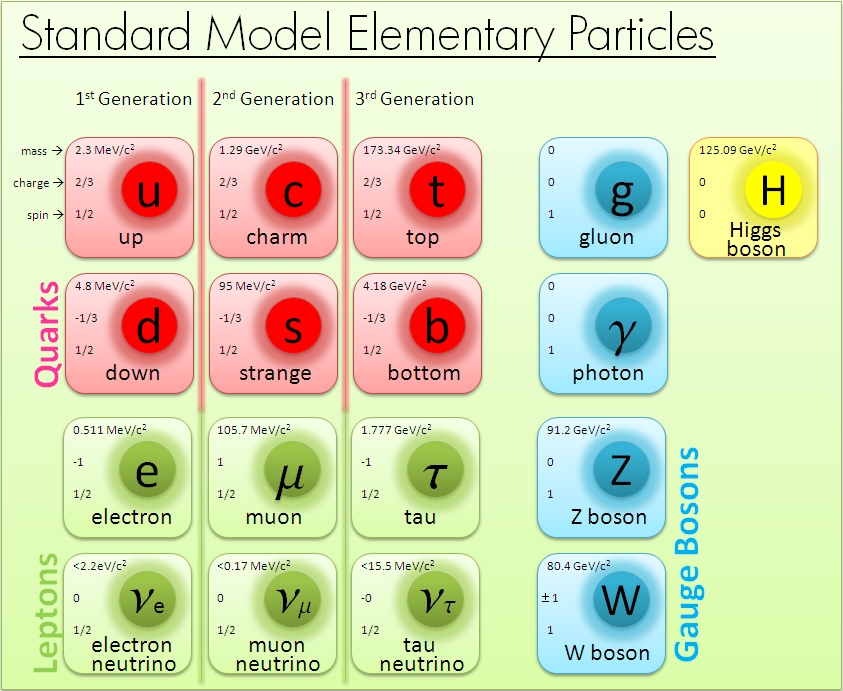
\includegraphics[width=5.2in]{Pictures/SM_elementary_particles.PNG}}
\caption {Chart of fundamental particles in the Standard Model of Particle Physics. There are three generations of leptons and three generations of quarks. Interactions are mediated by gauge bosons. The scalar Higgs field with its accompanying interaction carrier, the Higgs boson, gives mass to the leptons via spontaneous symmetry breaking in the Standard Model formulation.}
\label{fig:SM_particles}
\end{figure}

Although the SM has been very successful in its description of fundamental particle interactions, it is not considered satisfactory as a complete or fundamental theory. The SM description is given in terms of many free parameters which must be determined experimentally. These free parameters include all the fermion masses, the mass of the Higgs boson and the strength of the gauge couplings to mention a few. A great mystery of modern physics, the presence of dark matter and energy, is not accounted for in the SM. Perhaps its most glaring deficiency, however, is the total absence of gravity in the model. Because the strength of the gravitational force is many orders of magnitude lower than even the weak force (see Table \ref{tab:fundamental_forces}) this is not a problem for experimentalists; however, the complete absence of a force so fundamental to the existence of the universe as we know it and of life itself is a gaping hole in this otherwise beautiful model. Furthermore, in the SM neutrinos do not acquire mass via the Higgs mechanism and when it was found that they are not massless, their masses had to be inserted {\it ad hoc}.
\begin{table}[h]
\caption{Four fundamental forces of nature. Relative strengths are normalized to the energy regime where the strong force is close to unity. The values in this table were taken from {\it An Introduction to the Physics of Nuclei and Particles} by Richard Dunlop. Other resources quote slightly different relative strengths which can be attributed to the running of the coupling constants and the freedom to choose any energy scale for comparison.}
\begin{center}
\begin{tabular}{l|c|c|c|c}\hline
Force & Mediator & Charge & Strength & Range (fm)\\ \hline
Strong & gluon & color & 1 & 1\\
Electromagnetic & photon & electric & $10^{-2}$ & $\infty~(\frac{1}{r^2})$\\
Weak & $W^{\pm},~Z$ bosons & weak & $10^{-5}$ & $10^{-3}$\\
Gravity & graviton(undiscovered) & mass & $10^{-39}$ & $\infty~(\frac{1}{r^2})$\\
\hline
\end{tabular}
\end{center}
\label{tab:fundamental_forces}
\end{table}

Since the research in this thesis is mainly limited to electroweak physics and constitutes a test of electroweak predictions of the SM, the remainder of any theoretical discussions will be focused on the electroweak sector. 

\section{Electroweak Physics}
In 1961, Sheldon Glashow discovered a way to naturally combine the electric and weak interactions into a unified ``electroweak'' theory using an $SU(2)\times U(1)$ gauge group with four massless gauge bosons. Peter Higgs and others showed how fields can be made to acquire mass terms in a Lagrangian description by introducing a scalar field with a non-zero vacuum expectation value. Steven Weinberg and Abdus Salam independently condensed these ideas into a single model showing that through spontaneous symmetry breaking in non-Abelian gauge theories both massive and massless bosons are produced and that through the Higgs mechanism fermions naturally acquire mass. These seminal publications by Weinberg and Salam laid the foundations of the Standard Model\cite{Weinberg}\cite{Salam}.

One of the most important features of the SM relevant to the \Qs experiment is the phenomenon of parity violation, a phenomenon that was perhaps unsatisfactorily written into the model as opposed to arising naturally from it. Parity violation, the lack of symmetry in a physical process under spatial inversion, was known to be a signature of the charged weak interaction years before Weinberg and Salam published their early formulation of what is now the bedrock of the SM in 1967.  Ten years earlier Wu and collaborators had measured parity violation in weakly-mediated beta decays\cite{Wu} by observing that the measured decay rate of $^{60}$Co atoms was not symmetric with respect to the direction of a magnetic holding field. This was interpreted as a preference in nature towards left-handed neutrinos. Further experiments examining the decay of pions, $\pi^-\longrightarrow \mu^-+\bar{\nu_{mu}}$, were found to be consistent with a maximal violation of parity, that is, with no right-handed neutrino production\cite{Backenstoss}. Therefore, when Weinberg published his $SU(2)_L \times U(1)_Y$  formulation of electroweak theory, parity violation was simply included in the model by writing the left-handed electron and neutrino as a weak isodoublet and the right handed electron as an isosinglet\cite{Weinberg} as follows
\[
\left(\begin{array}{c}e^-\\\nu \end{array}\right)_L,~~~~~\left(e^-\right)_R.
\]
This model, although not widely accepted at first, solved a number of outstanding problems. First, it created mass for the fermions without imposing them {\it ad hoc} on a massless gauge theory, a process which was known to introduce non-renormalizable infinities. Second, by choosing a suitable gauge transformation, the unobserved massless Goldstone bosons were replaced by four bosonic fields: the massive charged boson field ($W^{\pm}$), a massive neutral boson field (Z), a massless neutral field ($\gamma$), and a ubiquitous, massive Higgs field. Two of these were interpreted as mediating known interactions: $\gamma$, the electromagnetic interaction, and $W^{\pm}$, the observed weak charged decays. The bold prediction of an unobserved massive neutral boson made this theory imminently testable. Six years later in 1973, neutral current processes were observed at CERN in the Gargamelle bubble chamber, validating a key claim of the Weinberg-Salam (W-S) electroweak model.  

Parity violation, although maximal for both charged and neutral weak currents in the W-S model, had not been confirmed in weak neutral current interactions, and many symmetric models predicted equal left and right-handed neutral weak currents\cite{Staley}. In 1977, two experiments attempting to measure parity violation in atomic transitions in bismuth published null results creating a dismal outlook for the W-S model\cite{Lewis}\cite{Baird}. Although the Weinberg model was considered the simplest, other ``hybrid'' models were created to account for parity violation including models with right-handed electron doublets paired with left-handed quark isospin doublets and right-handed quark isospin singlets. In 1978, Charles Prescott and collaborators published the results of electron-deuteron inelastic scattering in which they observed parity violation (non-zero at 10$\sigma$!) in the neutral-weak current, consistent with the simple Weinberg-Salam model \cite{Prescott}. The results of this experiment (E122) at SLAC, so established the W-S model that the following year Steven Weinberg, Abdus Salam and Sheldon Glashow shared the Nobel Prize in Physics ``for their contributions to the theory of the unified weak and electromagnetic interaction between elementary particles, including, inter alia, the prediction of the weak neutral current''\footnote{http://www.nobelprize.org/nobel\_prizes/physics/laureates/1979/}.

By the early 1970's non-Abelian gauge theories had been extended to include the strong interaction and the SM was established in its modern form and has remained nearly unchanged over the past four decades. Although known to be incomplete, the SM has stood up to a barrage of experimental tests over this period and, in almost every case, its predictions have proven to be correct. Parity violation was established as a key tool for probing weak physics processes and more recently as a precision test of key SM predictions.

One such experiment which utilized parity violation as a precision probe of electroweak physics is the recently completed \Qs experiment which ran in Hall C at Jefferson Lab in Newport News, VA, USA, from the Fall of 2010 to the Spring of 2012. This experiment ran with the intention of providing a first determination of the weak charge of the proton. The precision of this experiment also allows it to solidly test the ``running'' of the weak mixing angle, $\theta_W$, which is accurately predicted by the SM. Deviation from the predicted value can be interpreted as physics beyond the SM, whereas agreement with the predicted value would place constraints on some models of physics beyond the SM. 

The author was deeply involved in the setup, commissioning and running of the \Qs experiment and has been participating in data analysis over the 3+ years since the completion of the experimental data-taking phase in May 2012. The author's greatest contributions to the experiment have been in two main areas. First, building, commissioning and analyzing data for the laser system of the Compton polarimeter built specifically for \Qs and key to its small systematic error. Second, removing false asymmetries arising from helicity-correlated electron beam properties from the main data set. These topics will constitute the majority of this thesis.

The format of the thesis is as follows: 1). an introduction to the theory underlying the \Qs experiment and the motivation for the experiment. 2). an overview of the design of the experiment both from hardware and operational perspectives.
3). a detailed analysis of the authors contributions to Compton polarimetry and removal of false asymmetries and 4). a summary of the analysis steps to get from the raw measurement of a parity-violating asymmetry to the final result of the proton's weak charge. 
